\documentclass[../thesis.tex]{subfiles}

\begin{document}

\chapter{Benchmark}

\section{Aim}
The aim for benchmarking is understanding the performance characteristics of the proposed system under various loads and system configurations.

\section{Setup}

The hardware used for benchmarking is detailed in \autoref{sec:benchmarkingServer} and the critical technical specifications that affect the performance of the system are:
\begin{itemize}
	\item 8 Core 16 Threads
	\item 4.3 Ghz Clock Speed
	\item 32 GB Memory
	\item Hardware Virtualisation Enabled
\end{itemize}

To observe the performance characteristics of the proposed system with horizontal scalling, additional hardwares used for horizontal scalling benchmarking are listed below:
\begin{itemize}
	\item MacBook Pro 16 2019
		\begin{itemize}
			\item 8 Core 16 Threads
		\end{itemize}
	\item HP Envy dv6 2013
		\begin{itemize}
			\item 4 Core 8 Threads
		\end{itemize}
\end{itemize}


The software used for benchmarking is detailed in \autoref{sec:software} and the critical tehcnical specifications are:
\begin{itemize}
	\item Ubuntu 20.04
	\item Docker Engine Enabled
\end{itemize}

Additionally, the proposed system have two configrations that can be tweaked to show how the performance can be impacted:

\begin{itemize}
	\item Number of backend instances
	\item Number of async workers
\end{itemize}

The components of the proposed system are deployed to the benchmarking server using Docker Containers\footnote{A container virtualisation method, which allows the components to be run in an isolated environment that is always identical regardless of the environments of the server.} to manage the runtime dependencies. Note that this method of deployment have minimal impact of the performance of system. 

\section{Procedures}

\subsection{Limited Computational Resources}
The configurations listed in the table \ref{tab:lowsysconfbench} are used to observe the behaviours of the proposed system with limited computation resources that is comparable to a modern laptop.

\begin{table}[h!]
	\begin{center}
		\caption{A set of system configurations used for performance benchmarking with limited computational resources.}
		\label{tab:lowsysconfbench}
		\begin{tabular}{l|l|l}
			\toprule
			\textbf{No. Backend Instances} & \textbf{No. Async Workers} & \textbf{No. Devices}\\
			\midrule
			4 & 4 & 50\\
			4 & 4 & 100\\
			4 & 4 & 200\\
			\bottomrule
		\end{tabular}
	\end{center}
\end{table}

\subsection{Reasonable Computational Resources}

The configurations listed in the table \ref{tab:highsysconfbench} are used to observe the behaviours of the proposed system with reasonable computation resources that is comparable to a high performance consumer grade desktop computer system.

\begin{table}[h!]
	\begin{center}
		\caption{A set of system configurations used for performance benchmarking with reasonable computational resources.}
		\label{tab:highsysconfbench}
		\begin{tabular}{l|l|l}
			\toprule
			\textbf{No. Backend Instances} & \textbf{No. Async Workers} & \textbf{No. Devices}\\
			\midrule
			4 & 12 & 50\\
			4 & 12 & 100\\
			4 & 12 & 200\\
			\bottomrule
		\end{tabular}
	\end{center}
\end{table}

\subsection{Horizontal Scalling}

The proposed system is designed to scale, that is, having the capability of running multiple instances on multiple servers to distribute the load. The table \ref{tab:scalebench} shows the configurations used for benchmarking where there are three physically separated servers contributing to executing the tasks at the same time. The computation resources provided by the servers are shown in the table \ref{tab:computecontrib}

\begin{table}[h!]
	\begin{center}
		\caption{Contribution to computational resources.}
		\label{tab:computecontrib}
		\begin{tabular}{l|l|l|l}
			\toprule
			\textbf{Server} & \textbf{Threads} & \textbf{No. Backend} & \textbf{No. Workers}\\
			\midrule
			Benchmarking Server & 16 & 4 & 12\\
			MacBook Pro 16 2019 & 16 & 0 & 16\\
			HP Envy dv6 2013 & 8 & 0 & 8\\
			\bottomrule
		\end{tabular}
	\end{center}
\end{table}

\begin{table}[h!]
	\begin{center}
		\caption{A set of system configurations used for scalability benchmarking.}
		\label{tab:scalebench}
		\begin{tabular}{l|l|l}
			\toprule
			\textbf{No. Backend Instances} & \textbf{No. Async Workers} & \textbf{No. Devices}\\
			\midrule
			4 & 12 + 8 + 16 & 100\\
			4 & 12 + 8 + 16 & 200\\
			4 & 12 + 8 + 16 & 500\\
			4 & 12 + 8 + 16 & 1000\\
			\bottomrule
		\end{tabular}
	\end{center}
\end{table}

\subsection{Generating Loads}

The simulator is used to generate realisitic loads by spawning computer processes that are accssing the backend in the same manner as a real remote sensing device. For each simulated remote sensing device, it sends the sensing data to the backend every second for a total of 100 iterations to create a sustained load.

\subsection{Measuring Performance}

To quantify the performance, the response time of each request is measured and recorded. Once a simulated device has finished sending data, the response time for each iteration is saved to a CSV (Comma Seperated Values) file. Once all simulated devices have finished sending data, the average response time for each iteration across all simulated devices is calculated and saved to another CSV file. This is used to determine how well the backend handles various loads.

Note the performance of the backend can be determined by measuring the response time. However, the performance of the clients is hard to measure accuratly because the originating server may have different time as the client and the network delay also plays a big factor in the response time of the data update. Thus, the performance of the clients is determined subjectively, which is if the data is updated noticably slower than expected. 

\section{Analysis}

\subsection{Limited Computational Resources}

The average response time under different loads with limited computational resources is shown in the table \ref{tab:avg4-4}. From the table, it is clear the given loads did not saturate the backend since the response time for each load is considered very short. 

\begin{table}[h!]
	\begin{center}
		\caption{The average response time for the 4 backend and 4 async worker configuration.}
		\label{tab:avg4-4}
		\begin{tabular}{l|l}
			\toprule
			\textbf{No. Devs} & \textbf{Average Response Time}\\
			\midrule
			50 & 4.1 milliseconds\\
			100 & 4.89 milliseconds\\
			200 & 5.6 milliseconds\\
			\bottomrule
		\end{tabular}
	\end{center}
\end{table}

The preceived monitoring delay\footnote{The time it takes from the data is recorded in the sensing device, to the data is shown on the client.} with limited computational resources is shown in the table \ref{tab:delay4-4}. There is no preceivable delays for 50 and 100 devices. However, 200 devices introduced a significant monitoring delay of up to three minutes. That means, it takes three minutes for a data to show up on the client since it is recorded at the sensing device. We also know the fact that the backend is no where near its saturation point with a load generated by 200 devices. The only possible bottlenecks here is the four async workers are struggling to process 200 data insertion requests per second, because the data insertion requests are handled by the async workers, not the backend itself, as inserting data into the database is considered time insensitive in this scenario. Additionally, the data updates are only generated until the async worker successfully insert the data into the database, which explains the significant delay in receiving updates at the clients. 

\begin{table}[h!]
	\begin{center}
		\caption{The preceived monitoring delay for the 4 backend and 4 async worker configuration.}
		\label{tab:delay4-4}
		\begin{tabular}{l|l}
			\toprule
			\textbf{No. Devs} & \textbf{Preceived delay}\\
			\midrule
			50 & No delay \\
			100 & No delay\\
			200 & Delayed up to 3 mins\\
			\bottomrule
		\end{tabular}
	\end{center}
\end{table}

The figure \ref{fig:4-4} shows the response time for each iteration under different load scenarios. The figure suggests there is no positive or negative associations between the response time and the number of iterations. That means the response time is expected to stay at the same level regardless of the number of iterations and showing no signs of performance degradation. 

\begin{figure}[!ht]
	\centering
	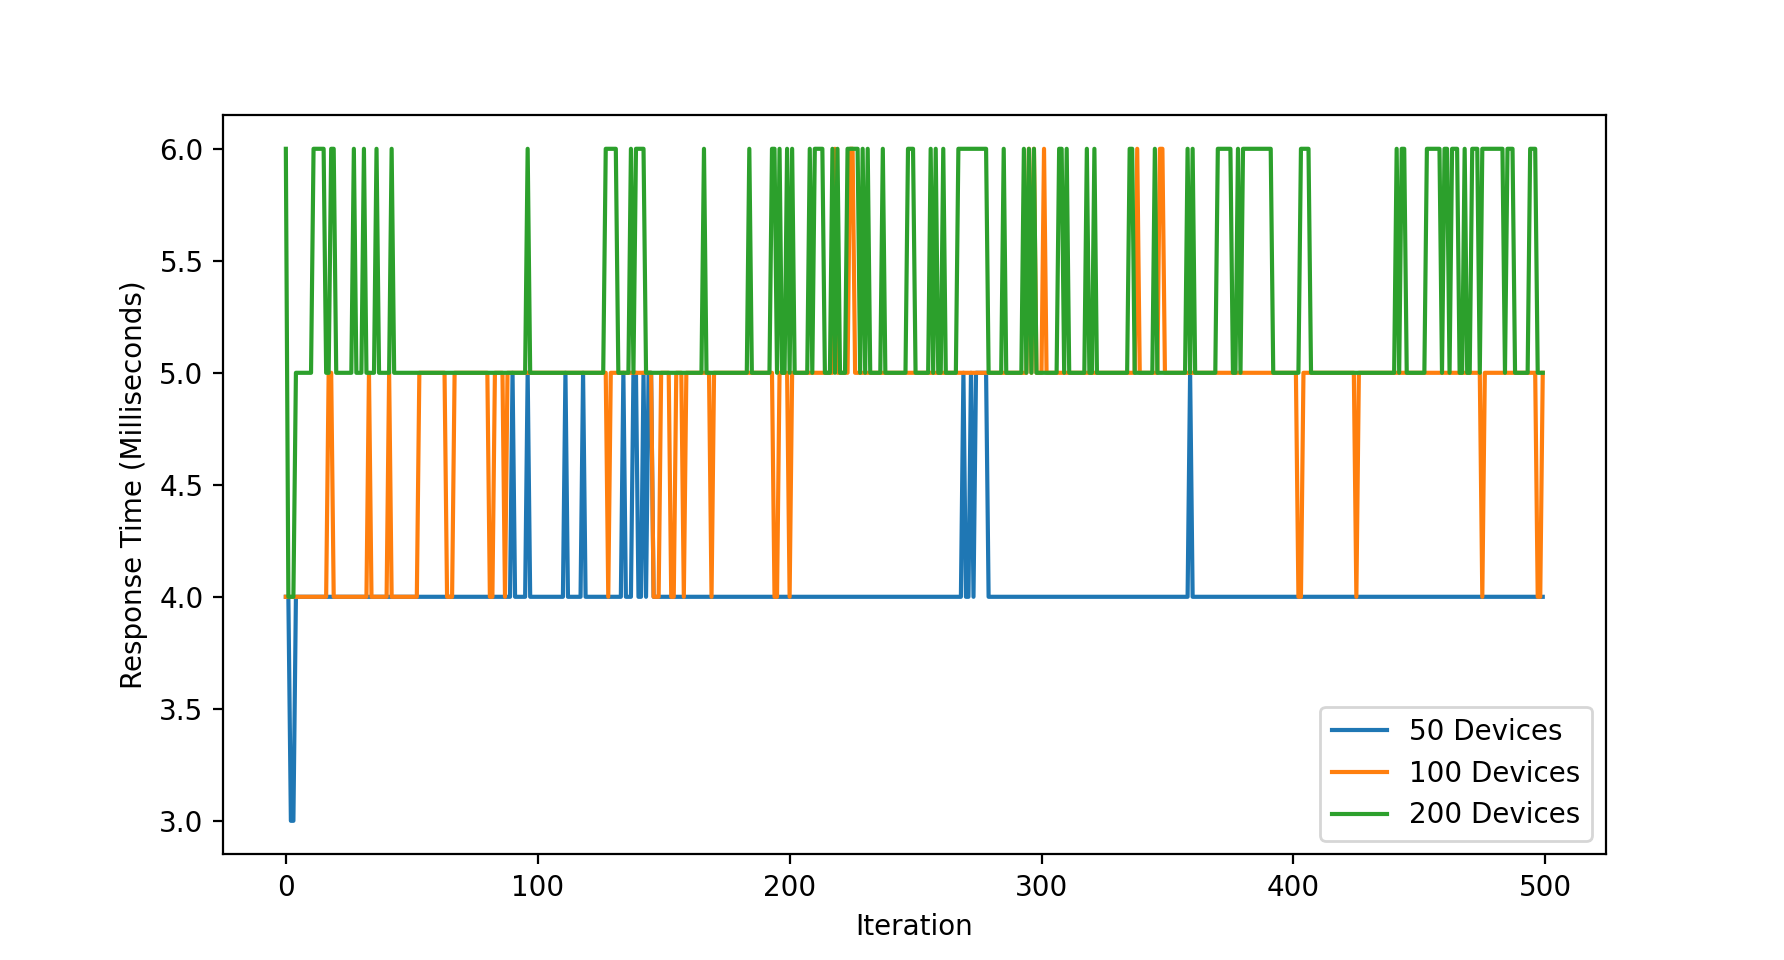
\includegraphics[width=0.8\linewidth]{4-4.png}
	\caption{The response time for each iteration using the 4 backend and 4 async worker configuration.}
	\label{fig:4-4}
\end{figure}

With the evidences presented above, the 4 backend and 4 async worker configuration is expected to serve around 100 devices for a long period of time without introducing delays or significant performance degredation. 

\subsection{Reasonable Computational Resources}

\begin{figure}[!ht]
	\centering
	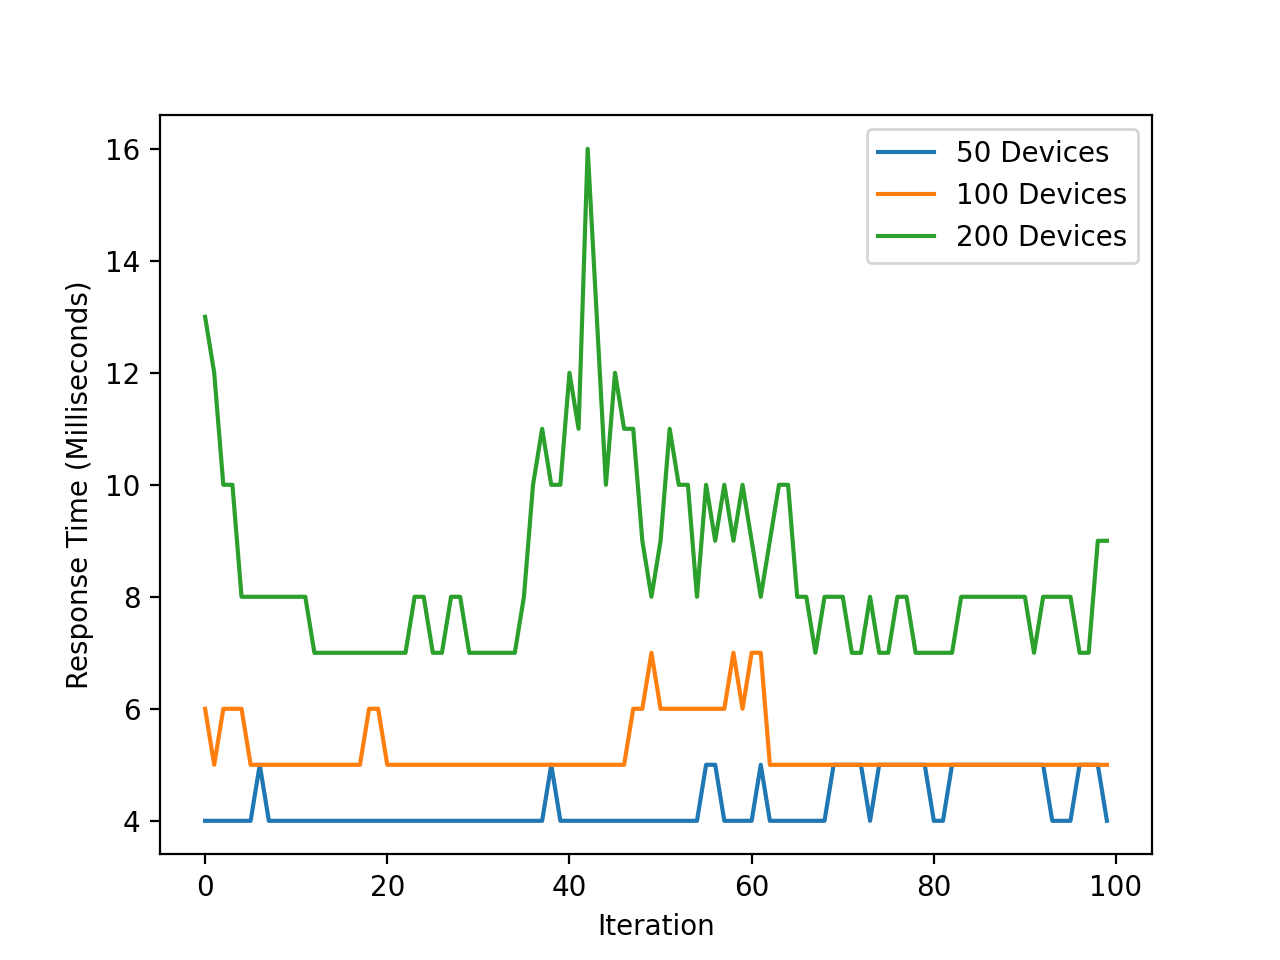
\includegraphics[width=0.8\linewidth]{4-12.png}
	\caption{The response time for each iteration using the 4 backend and 12 async worker configuration.}
	\label{fig:4-12}
\end{figure}

\subsection{Horizontal Scalling}

\begin{figure}[!ht]
	\centering
	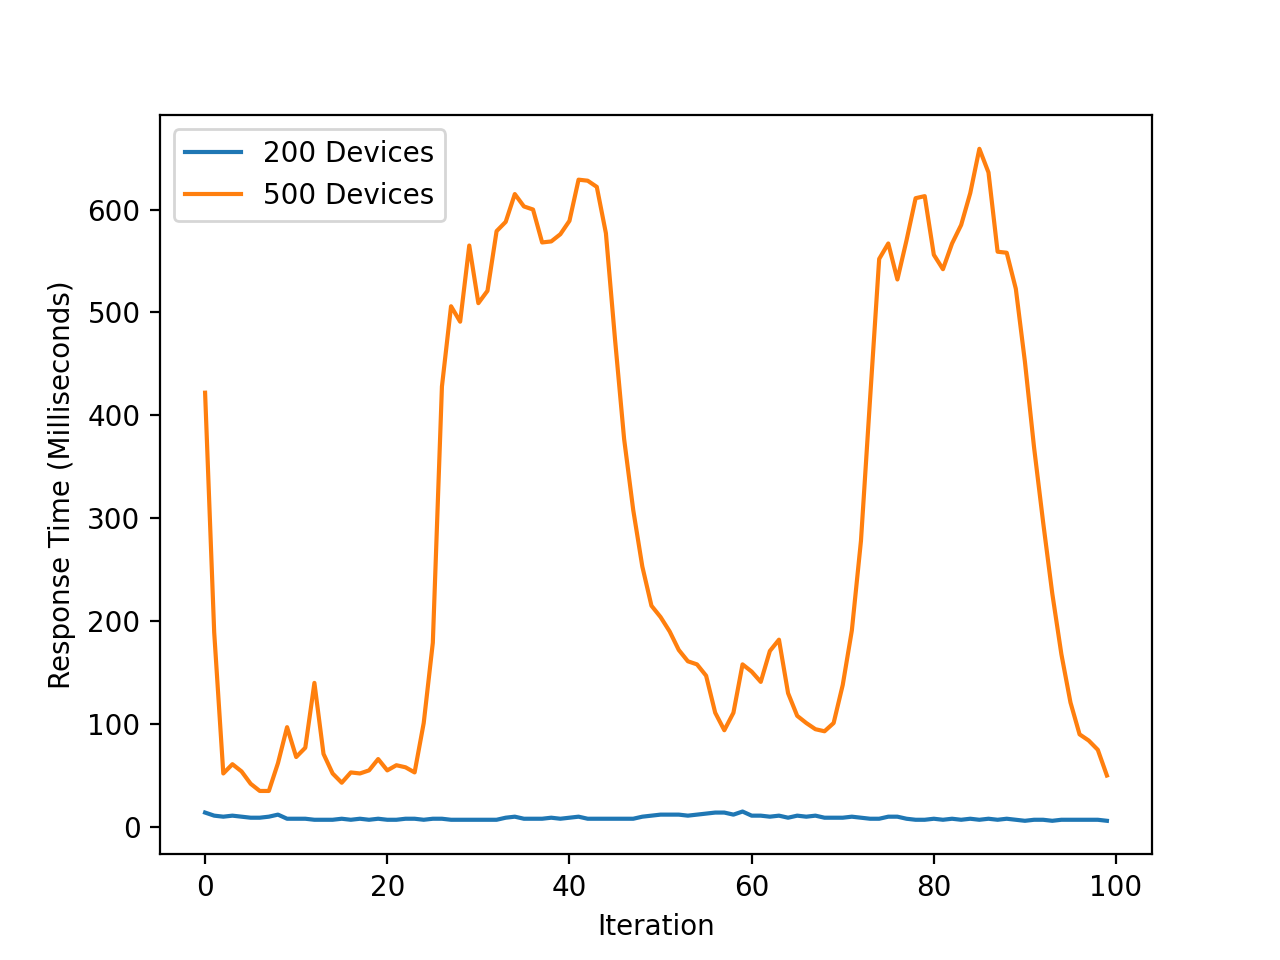
\includegraphics[width=0.8\linewidth]{4-36.png}
	\caption{The response time for each iteration using the 4 backend and 12 + 8 + 16 async worker configuration.}
	\label{fig:4-36}
\end{figure}

\begin{figure}[!ht]
	\centering
	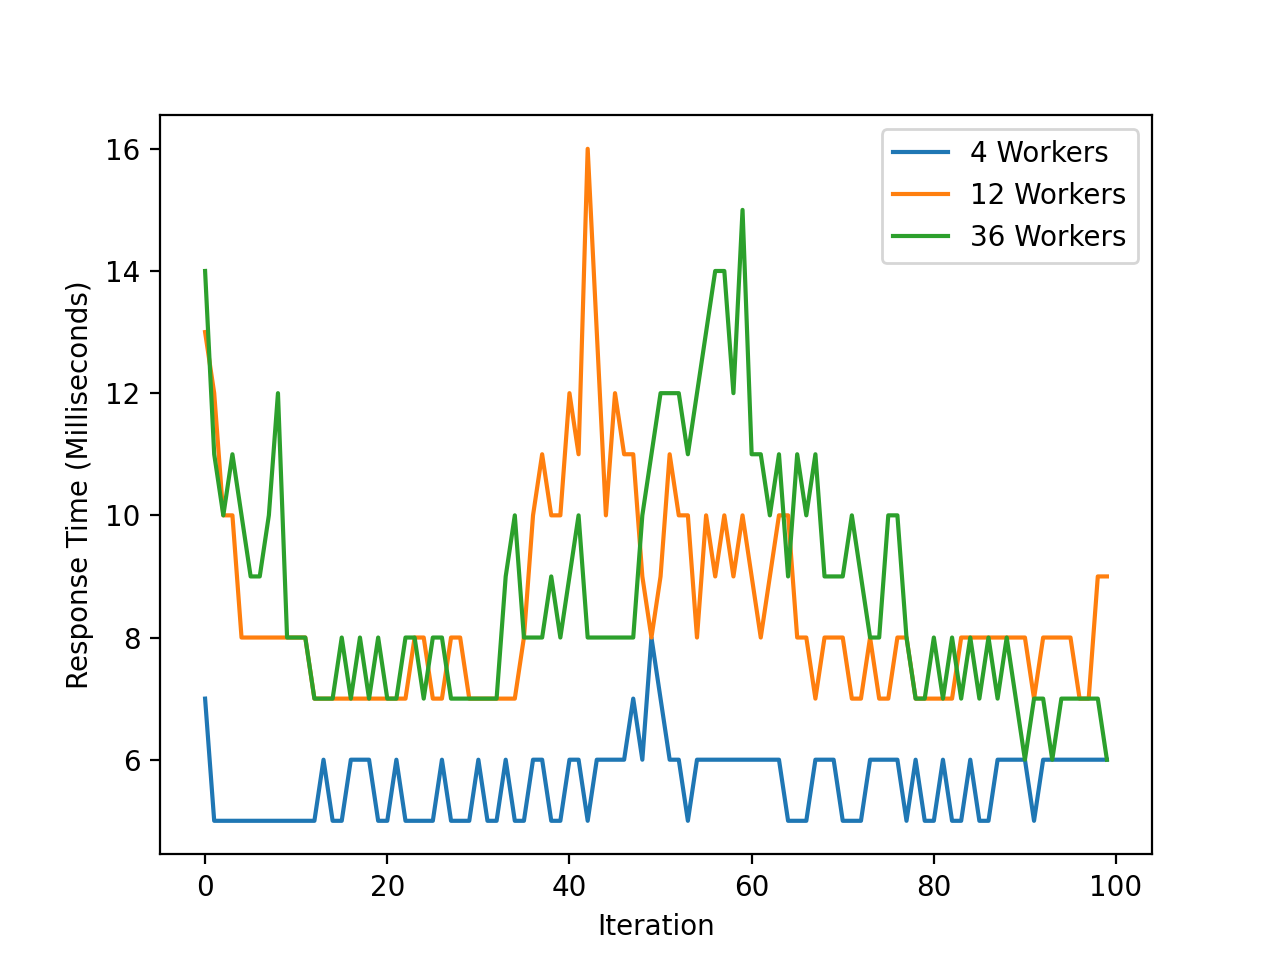
\includegraphics[width=0.8\linewidth]{w-4-12-36.png}
	\caption{The response time for each iteration for 200 devices in 4, 12, and 36 workers configuration.}
	\label{fig:w-4-12-36}
\end{figure}



\end{document}